% ------------------------------------------------------------------------------
% TYPO3 Version 9.4 - What's New (Dutch Version)
%
% @license	Creative Commons BY-NC-SA 3.0
% @link		https://typo3.org/help/documentation/whats-new/
% @language	Dutch
% ------------------------------------------------------------------------------

\section{Wijzigingen voor integrators}
\begin{frame}[fragile]
	\frametitle{Wijzigingen voor integrators}

	\begin{center}\huge{Hoofdstuk 2:}\end{center}
	\begin{center}\huge{\color{typo3darkgrey}\textbf{Wijzigingen voor integrators}}\end{center}

\end{frame}

% ------------------------------------------------------------------------------
% #85256 - Install TYPO3 on SQLite

\begin{frame}[fragile]
	\frametitle{Wijzigingen voor integrators}
	\framesubtitle{TYPO3 installeren op SQLite (1)}

	\begin{itemize}
		\item TYPO3 ondersteunt nu \href{https://www.sqlite.org}{SQLite},
			een autonoom, lichtgewicht open source SQL database-systeem
		\item SQLite kan gekozen worden tijdens webgebaseerde installatie,
			als de PHP-module "pdo\_sqlite" is geïnstalleerd en ingeschakeld:
	\end{itemize}

	\begin{figure}
		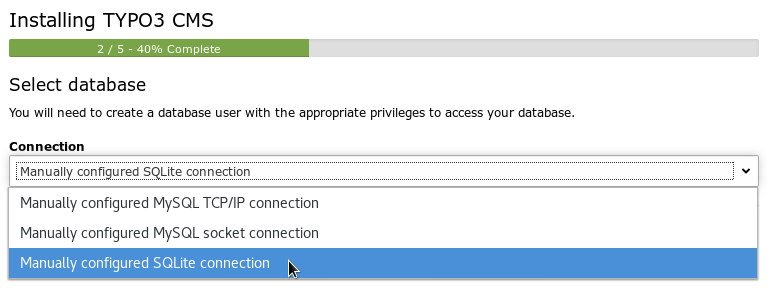
\includegraphics[width=0.65\linewidth]{ChangesForIntegrators/85256-InstallTYPO3OnSQLite.png}
	\end{figure}

\end{frame}

% ------------------------------------------------------------------------------
% #85256 - Install TYPO3 on SQLite

\begin{frame}[fragile]
	\frametitle{Wijzigingen voor integrators}
	\framesubtitle{TYPO3 installeren op SQLite (2)}

	\begin{itemize}
		\item Database is opgeslagen in een enkel bestand, wat betekent dat
			TYPO3 installaties nu met alleen PHP kunnen werken, inclusief dataopslag
		\item SQLite gebruiken is zinvol voor kleine TYPO3 sites of voor
			testen en ontwikkelen
		\item Systeembeheerders moeten de juiste maatregelen nemen om het
			\texttt{*.sqlite} bestand te beschermen tegen ongeoorloofde toegang als het bestand
			 binnen de webroot wordt opgeslagen (afhankelijk van soort installatie)
	\end{itemize}

\end{frame}

% ------------------------------------------------------------------------------
% #85947 - Page based URL handling

\begin{frame}[fragile]
	\frametitle{Wijzigingen voor integrators}
	\framesubtitle{URL-afhandeling voor pagina's}

	\begin{itemize}
		\item Alle links gemaakt in de backend en fronten gebruiken dit veld,
			indien gevuld
		\item URL-afhandeling voor pagina's vereist een Site-configuratie
	\end{itemize}

	\begin{figure}
		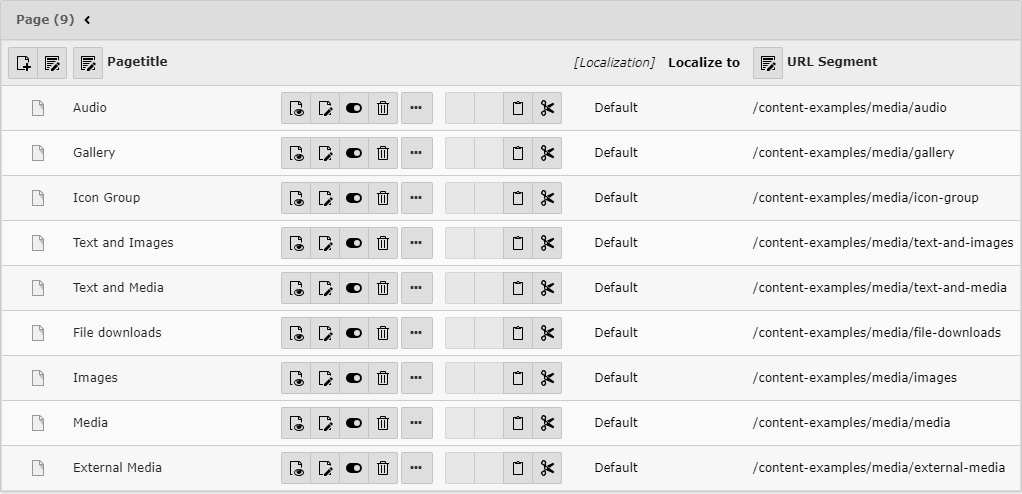
\includegraphics[width=0.7\linewidth]{ChangesForIntegrators/xxxxx-UrlSegments.png}
	\end{figure}

\end{frame}

% ------------------------------------------------------------------------------
% #84729 - New TCA type "slug"

\begin{frame}[fragile]
	\frametitle{Wijzigingen voor integrators}
	\framesubtitle{URL-afhandeling voor pagina's}

	% decrease font size for code listing
	\lstset{basicstyle=\smaller\ttfamily}

	\begin{itemize}
		\item Een nieuw TCA-veldtype \texttt{slug} is toegevoegd
		\item Definieer delen van een URL-pad voor het genereren en oplossen van URL's

		\begin{lstlisting}
'type' => 'slug',
'config' => [
  'generatorOptions' => [
    'fields' => ['title', 'nav_title'],
    'fieldSeparator' => '/',
    'prefixParentPageSlug' => true
  ]
  'fallbackCharacter' => '-',
  'eval' => 'uniqueInSite'
]
		\end{lstlisting}
	\end{itemize}

\end{frame}

% ------------------------------------------------------------------------------
% #44297 - Interval presets for cron command of scheduler task

\begin{frame}[fragile]
	\frametitle{Wijzigingen voor integrators}
	\framesubtitle{Taakplanner}

	\begin{itemize}
		\item Voorkeuzes zijn toegevoegd aan de Taakplanner:

			\begin{itemize}
				\item \texttt{0 9,15 * * 1-5}\tabto{3.8cm}(ma tot vr om 9:00 en 15:00)
				\item \texttt{0 */2 * * *}\tabto{3.8cm}(elke 2 uur)
				\item \texttt{*/20 * * * *}\tabto{3.8cm}(elke 20 minuten)
				\item \texttt{0 7 * * 2}\tabto{3.8cm}(elke dinsdag om 7:00)
			\end{itemize}

	\end{itemize}

	\begin{figure}
		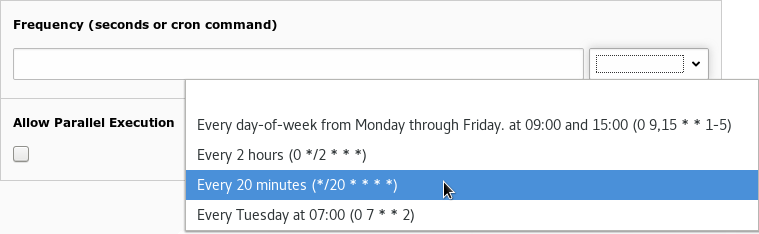
\includegraphics[width=0.80\linewidth]{ChangesForIntegrators/44297-IntervalPresetsInSchedulerTask.png}
	\end{figure}

\end{frame}

% ------------------------------------------------------------------------------
% #83476 - Load merged JS files asynchronous
% #85146 - Read environment variables in TypoScript

\begin{frame}[fragile]
	\frametitle{Wijzigingen voor integrators}
	\framesubtitle{TypoScript wijzigingen/verbeteringen (1)}

	% decrease font size for code listing
	\lstset{basicstyle=\smaller\ttfamily}

	\begin{itemize}
		\item De script-tag van samengevoegde JS bestanden krijgt het \texttt{async} attribuut
		 als alle bestanden het attribuut \texttt{async} hebben in TypoScript:

			\begin{lstlisting}
config.concatenateJs = 1
page = PAGE
page.includeJSFooter {
  test = path/to/file.js
  test.async = 1
}
			\end{lstlisting}

		\item Het is mogelijk om omgevingsvariabelen uit te lezen in TypoScript:

			\begin{lstlisting}
# Definieer standaardwaarde
myConstant = defaultValue
# Schakel overschrijven door omgevingsvariabele in
myConstant := getEnv(MYCONSTANT)
			\end{lstlisting}

	\end{itemize}

\end{frame}

% ------------------------------------------------------------------------------
% #85550 - Add context check for TypoScript

\begin{frame}[fragile]
	\frametitle{Wijzigingen voor integrators}
	\framesubtitle{TypoScript wijzigingen/verbeteringen (2)}

	% decrease font size for code listing
	\lstset{basicstyle=\smaller\ttfamily}

	\begin{itemize}
		\item De nieuwe Context API (zie "Wijzigingen voor ontwikkelaars")
			zorgt ervoor dat integrators dit ook kunnen gebruiken in TypoScript

		\item Voorbeeld:

			\begin{lstlisting}
10 = TEXT
10.data = context:workspace:id
			\end{lstlisting}

		\item Syntax is: \texttt{context:[aspectName]:[propertyName]}

		\item Array's worden automatisch omgezet in kommagescheiden lijsten\newline
			\smaller(ideaal voor bijvoorbeeld het uitlezen van details van gebruikersgroepen)\normalsize

	\end{itemize}

\end{frame}

% ------------------------------------------------------------------------------
% #86057 - Improved typolink / URL link generation

\begin{frame}[fragile]
	\frametitle{Wijzigingen voor integrators}
	\framesubtitle{TypoScript wijzigingen/verbeteringen (3)}

	% decrease font size for code listing
	\lstset{basicstyle=\smaller\ttfamily}

	\begin{itemize}
		\item Met de nieuwe site-gebaseerde afhandeling is de standaard \texttt{GET}-parameter
			"L" nu overbodig
		\item Een nieuwe parameter \texttt{typolink.language} is toegevoegd

			\begin{lstlisting}
page.10 = TEXT
page.10.value = Link naar pagina met ID van huidige taal
page.10.typolink.parameter = 23
page.20 = TEXT
page.20.value = Link naar pagina met de ID van taal 3
page.20.typolink.parameter = 23
page.20.typolink.language = 3
			\end{lstlisting}

	\end{itemize}

\end{frame}

% ------------------------------------------------------------------------------
% #85196 - Unify simulate user settings for Backend admins

\begin{frame}[fragile]
	\frametitle{Wijzigingen voor integrators}
	\framesubtitle{Simuleer gebruiker bij BE gebruikersinstellingen}

	\begin{itemize}
		\item Admin-gebruikers hadden de mogelijkheid om te wisselen naar een andere
			backend gebruiker ("Gebruikersinstellingen → Simuleer backend gebruiker")
		\item Deze functie is verwijderd
	\end{itemize}

	\begin{figure}
		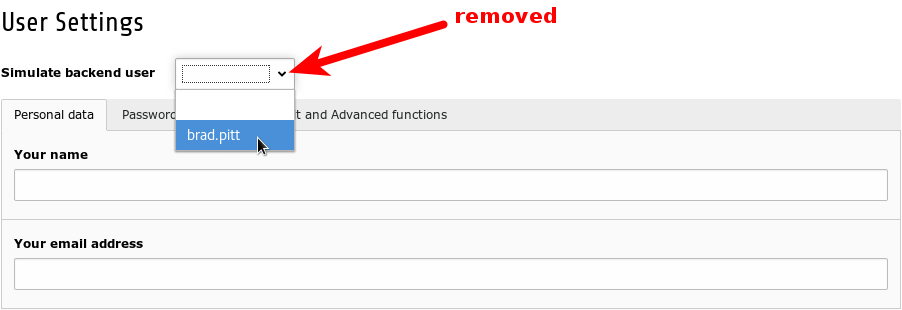
\includegraphics[width=0.80\linewidth]{ChangesForIntegrators/85196-SimulateUserRemovedForAdmins.png}
	\end{figure}

\end{frame}

% ------------------------------------------------------------------------------
% #84133 - Introduce variants

\begin{frame}[fragile]
	\frametitle{Wijzigingen voor integrators}
	\framesubtitle{Voorwaardelijke varianten in \texttt{EXT:form} (1)}

	\begin{itemize}
		\item Nieuwe optie voor extensie "Formulieren": \textit{voorwaardelijke varianten}
		\item Varianten kunnen voorwaarden bevatten waarmee eigenschappen van een formulierelement
			gewijzigd kunnen worden
		\item Dit maakt het mogelijk om formulierelementen, validaties en opties van eindacties aan
			te passen op basis van voorwaarden

	\end{itemize}

\end{frame}

% ------------------------------------------------------------------------------
% #84133 - Introduce variants

\begin{frame}[fragile]
	\frametitle{Wijzigingen voor integrators}
	\framesubtitle{Voorwaardelijke varianten in \texttt{EXT:form} (2)}

	\begin{itemize}
		\item Typische toepassingen zijn bijvoorbeeld:

			\begin{itemize}
				\item Vertaal waarden van een formulierelement gebaseerd op de
					huidige taal
				\item Voeg validaties toe en verwijder ze afhankelijk van de waarde
					van een ander element
				\item Stel waardes van eindactie in afhankelijk van de waarde van een element.
				\item Verberg een formulierelement in bepaalde eindacties en op de samenvattigspagina.
				\item Verberg hele pagina's afhankelijk van de waarde van een formulierelement.
				\item etc.
			\end{itemize}

		\item \href{https://docs.typo3.org/typo3cms/extensions/form}{Officiële documentatie}
			bevat meer details en voorbeelden

	\end{itemize}

\end{frame}

% ------------------------------------------------------------------------------
% #85355 - Support basic HTML5 fields in FormEngine

\begin{frame}[fragile]
	\frametitle{Wijzigingen voor integrators}
	\framesubtitle{HTML5 validatie in Backend velden}

	\begin{itemize}
		\item HTML5-specifieke veldtypes en attributen worden nu gebruikt door
			de FormEngine in de TYPO3 backend
		\item Hieronder vallen e-mail, getallen, incl. bereik, etc.
		\item HTML-tagattributen zijn gebaseerd op de \texttt{eval} TCA-configuratie
		\item Hiermee kan aangepaste JavaScript afhandeling in de toekomst verdwijnen
	\end{itemize}

\end{frame}

% ------------------------------------------------------------------------------
% #86001 - Regular Workspace cleanup tasks available via CLI commands

\begin{frame}[fragile]
	\frametitle{Wijzigingen voor integrators}
	\framesubtitle{Werkruimte CLI commando's}

	% decrease font size for code listing
	\lstset{basicstyle=\small\ttfamily}

	\begin{itemize}
		\item TYPO3 ondersteunt twee nieuwe, op Symfony gebaseerde CLI commando's
			om gewone taken af te vuren:

			\begin{itemize}

				\item \texttt{workspace:autopublish}\newline
					Controleert op werkruimtes met configurie voor automatisch publiceren
					en voert een publicatie/wissel-proces uit.
					\newline

				\item \texttt{cleanup:previewlinks}\newline
					Verwijdert verlopen links naar voorvertoningen opgeslagen in sys\_preview
					uit de database.

			\end{itemize}

		\item Aanroep op de commandoregel, bijvoorbeeld:

			\begin{lstlisting}
$ typo3/sysext/core/bin/typo3 workspace:autopublish
			\end{lstlisting}

	\end{itemize}

\end{frame}

% ------------------------------------------------------------------------------
% #81430 - Improve TS Template module information on root level list

\begin{frame}[fragile]
	\frametitle{Wijzigingen voor integrators}
	\framesubtitle{Informatie in TypoScriptmodule}

	\begin{itemize}
		\item Overzicht van TypoScript-sjabolen op de rootpagina is herschreven
		\item HTML uitvoer op basis van Fluid
		\item Informatie omvat paginanaam, sjabloonnaam (met link om het record te bewerken)
			, status (icoon), root/uitbreidingssjabloon

	\end{itemize}

	\begin{figure}
		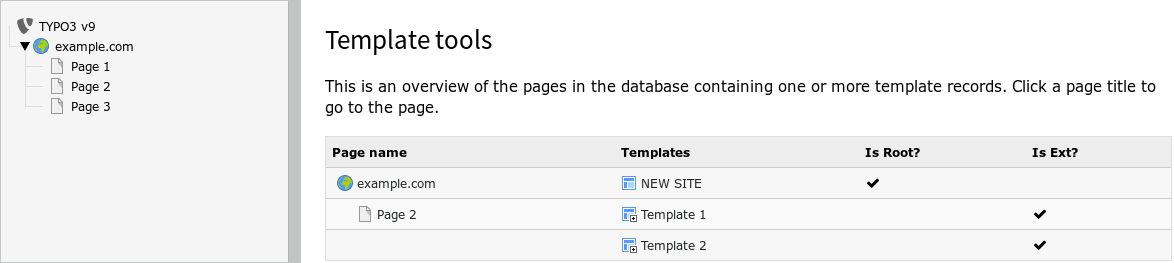
\includegraphics[width=0.80\linewidth]{ChangesForIntegrators/81430-TypoScriptModuleInformation.png}
	\end{figure}

\end{frame}

% ------------------------------------------------------------------------------
% #85393 - Only import extensions from 2015+ into EM

\begin{frame}[fragile]
	\frametitle{Wijzigingen voor integrators}
	\framesubtitle{Extensies}

	\begin{itemize}
		\item Extensies van voor 10 november 2015 (TYPO3 v7 LTS) worden uitgesloten
			bij de import van de lijst extensies
		\item Dit reduceert de databasetabel met ongeveer 75\%
	\end{itemize}

\end{frame}

% ------------------------------------------------------------------------------
